\documentclass[project2.tex]{subfiles}
\begin{document}
\subsection{A Dual Queueing Model}
\paragraph{}
Mathematical modelling is used to capture the most intrinsic fact of a real problem into a stochastic framework. For this reason, mathematicians sometimes find out that they can use same model to describe different facts which seem to have less in common. Mathematical models are rather universal. A concrete example is that we can use the ruin theory to analyse a single server with exponential inter-arrival times quest and arbitrary service time distribution. In this section, we will first point out  where they are equivalent and use the behaviour of the server to derive the ruin probability reversely.
\subsubsection{Queuing model and waiting time}
\paragraph{}
The server mentioned above in reality is like a clinic with one doctor. Patients come to the clinic follow some random patterns and they have to wait for previous patients to finish their diagnosis first. The doctor spends different times on patients. The most interesting problem is that each patient has to spend how much time in the waiting room. This kind of problem has a special name in mathematics which is called the queuing theory. We will first give the explicit model of this clinic.
\begin{definition}
Queuing model
\end{definition}
\begin{itemize}
\item The diagnosis time of different patients are independent and both follow the same distribution $F_U$. $U_i$ stands for the diagnosis time of i-th patient.
\item The inter-arrival time between i and i+1 patients are $\beta T_i$. $\{T_i\}$ are i.i.d exponentially distributed with parameter $\lambda$.
\item Doctor never rests except there are no patients waiting.
\item Patients are treated in order of arrival. Once the patients come, they have to stay in the waiting room till all the previous patients over. The waiting room has infinite space.   
\item $L_i$ is the just time that $i+1$th patient has to stay in the waiting room and $L_0=0$. 
\end{itemize}
\paragraph{}
It can be easily figure out that the waiting time of patients follow the recurrence relation.
$$L_n=(L_{n-1}+U_n-\beta T_n)_+$$
And the rounding to zero part is because the inter-arrival time may be very big to make $L_i$ be negative i.e. the doctor finishes all his/her patients before new patient arrives, but $L_i$ is the waiting time has minimum 0 so we round out the negative part and this part is actually the rest period of the doctor between two arrival.
\subsubsection{Elegant relation}
\begin{lemma}
Suppose $Y_i=U_i-\beta T_i$,
$$L_n=max(0,Y_n,Y_{n-1}+Y_n,...,Y_n+...Y_2+Y_1)$$
\end{lemma}
\begin{proof}
The intuitive solution is just $\sum_{i=1}^nY_i$ but it is wrong since the waiting time can not be negative and $Y_i$ can be negative so $L_n$ can not simply be that form. Now we consider the situation $L_i=0$ i.e. the i+1 patient comes and finds that he needs not to wait for anybody and assume all the patients i+2,i+3,...n has to wait. Then the rounding to zero part in the recurrence relation above is not applied. And $L_n$ is  just $Y_{i+1}+Y_{i+2}...+Y_n$. In reality, i can only be one of 0,1,2...n so $L_n$ is one of $$(0,Y_n,Y_{n-1}+Y_n,...,Y_n+...Y_2+Y_1)$$
\paragraph{}
To figure out which one is $L_n$, we first assume the solution is $Y_{i+1}+Y_{i+2}...+Y_n$ as previous assumption. The solution is true when $L_i=0$ and all the patients i+2,i+3,...n has to wait. That is to say, the doctor does not have the time to rest so $\sum_{k=i+1}^{j<n}Y_k\geq 0$ thus $L_n=Y_{i+1}+Y_{i+2}...+Y_n=\sum_{k=i+1}^{j<n}Y_k+\sum_{k=j+1}^{n}Y_k$ implies $$(Y_{i+2}+Y_{i+3}...+Y_n,Y_{i+3}...+Y_n,...,Y_n)=\sum_{k=j+1}^{n}Y_k,j=i...n-1\leq L_n$$
\paragraph{}
Now we trace back all the waiting time of previous patients. Somebody may have zero waiting time or everybody has to wait (except the first patient). If every body has to wait then $\sum_{k=1}^{j<i}Y_k\geq 0$ but $\sum_{k=1}^{i}Y_k\leq 0$ since $L_i=0$ so $\sum_{k=j}^{i}Y_k\leq 0$ thus $L_n$ implies $$(Y_{1}+Y_{2}...+Y_n,Y_{2}...+Y_n,...,Y_{i-1}+Y_n)=L_n+\sum_{k=j}^{i}Y_k\leq L_n$$ 
\paragraph{}
If some previous patients have zero waiting time, let $w=argsup\{L_p=0,p<i\}$ we find $L_w=0$ which means the w+1 patient has zero waiting time and all patient between w+1 and i+1 has to wait. It is just like the situation of  previous  paragraph if we see w+1 as 1. Thus, $$(Y_{w+1}+Y_{w+2}...+Y_n,Y_{w+2}...+Y_n,...,Y_{i-1}+Y_n)\leq L_n$$
\paragraph{}
Further consider $w_{-1}=argsup\{L_p=0,p<w<i\}$, we can fold the time line making w and i coincide and $w_{-1}$ is just like w in previous paragraph. This trick can be applied to both $w_{-1},w_{-2}.....$ so $$(Y_{1}+Y_{2}...+Y_n,Y_{2}...+Y_n,...,Y_{i-1}+Y_n)\leq L_n$$
\paragraph{}
Since i is not fixed and for any i, $L_n$ will the the max of the possible values. It follows that 
$$L_n=max\{0,Y_n,Y_{n-1}+Y_n,...,Y_n+...Y_2+Y_1\}$$
\end{proof} 
\begin{lemma}for all n=1,2...
$$(Y_n,Y_{n-1}+Y_n,...,Y_n+...Y_2+Y_1)\overset{d}{=}(Y_1,Y_{1}+Y_2,...,Y_1+...Y_{n-1}+Y_n)$$
\end{lemma}
\begin{proof}Since both $\{U_i,i\geq 1\}$ and $\{T_i,i\geq 1\}$ are i.i.d themselves and $\beta$ is just a constant, we have $\{Y_i,i\geq 1\}$ are i.i.d.. From the definition of joint distribution, we have
\footnotesize{
\begin{align*}
&P(Y_1\in A_1,Y_1+Y_2\in A_2,Y_1+Y_2+Y_3\in A_3,...,Y_1+...Y_{n-1}+Y_n \in A_n)\\
&=P(Y_1\in A_1)P(Y_1+Y_2\in A_2|Y_1\in A_1)P(Y_1+Y_2+Y_3\in A_3|Y_1+Y_2\in A_2,Y_1\in A_1)...\\
&=P(Y_n\in A_1)P(Y_n+Y_{n-1}\in A_2|Y_n\in A_1)P(Y_n+Y_{n-1}+Y_{n-2}\in A_3|Y_n+Y_{n-1}\in A_2,Y_n\in A_1)...\\
&=P(Y_n\in A_1,Y_n+Y_{n-1}\in A_2,Y_n+Y_{n-1}+Y_{n-2}\in A_3,...,Y_n+...Y_2+Y_1 \in A_n)
\end{align*}
}
\end{proof}
\begin{theorem}
Recall definition of $W_n$ and M in section 1.3. Then, $$P(L_n>u)=P(\underset{1\leq i\leq n}{sup}W_i>u)$$ 
$$\lim_{n\rightarrow\infty}P(L_n>u)=P(\underset{i\geq1}{sup}\hspace{4pt} W_i>u)=P(M>u)=\varphi(u)$$  
\end{theorem}
\begin{proof}
\begin{align*}
P(L_n>u)&=P(max\{0,Y_n,Y_{n-1}+Y_n,...,Y_n+...Y_2+Y_1\}> u)\\
&=P(max\{0,Y_1,Y_1+Y_2,...,Y_1+...Y_{n-1}+Y_n\}>u)\\
&=P(max\{S'_1,S'_1+S'_2,...,S'_1+...S'_{n-1}+S'_n\}>u)\\
&=P(\underset{1\leq i\leq n}{sup}\hspace{4pt} W_i>u)
\end{align*}
\paragraph{}
Since $max\{0,Y_1,Y_1+Y_2,...,Y_1+...Y_{n-1}+Y_n\}\leq max\{0,Y_1,Y_1+Y_2,...,Y_1+...Y_{n-1}+Y_n+Y_{n+1}\}$ so $P(L_n>u)\leq P(L_{n+1}>u)\leq 1$. Thus, {\it monotone convergence theorem }yields the second equation of the theorem.
\paragraph{}
This clinic is somehow a insurance company! The waiting time of the transfinite patient bigger than u is just the probability of ultimate ruin. Of course, the doctor is free from karoshi. This clinic model can be modify to a M/G/1 queue, which has been studied extensively. 
\end{proof}     
\subsection{M/G/1 Queue}
\paragraph{}
Queuing theory is developed to study the behaviour of waiting lines. In this theory, we construct a mathematical model so as to predict the queue length(number of customers in system) and waiting time of the system in interest. A queueing node can be classified using {\it Kendall's notation} in the form A/S/C where A describes the time of inter-arrivals to the queue, S the size of job (service time) and C the number of servers at the node.    
\subsubsection{Basic definition and property}
\begin{definition}
M/G/1 queue
\begin{equation*}
\left\{
\begin{array}{lcl}
M:\text{Markov or memoryless, arrivals occur as a Poisson process with rate $\lambda$}\\
G:\text{General service time distribution with E[S]=$u^{-1}$}\\
1:\text{Single server}\\
\end{array} 
\right.
\end{equation*}
\end{definition}
\paragraph{}
To analyse the average time spent in this M/G/1 queue by a customer(arriver) and the average number of customer in this system, we have to introduce three useful property of M/G/1 system which are {\it Little's Law, Level Crossing Low and PASTA}. We assume the queue length is bounded and the system will reach a equilibrium, and mainly focus on the behaviour of the system in equilibrium.

Let A(t) be the number of arrivals to the system in [0,t] and D(t) be the departure. Then, N(t), the number of customers in the system (both in service and waiting) can be expressed as $$N(t)=A(t)-D(t)+N(0)$$ where N(0) is the number of customers at time 0. We often assume system is initially empty i.e. N(0)=0 and operates in a way such that N(t)=o(A(t)) thus $$\lim_{t\rightarrow\infty}\frac{N(t)}{A(t)}=0$$ And $T_i$ be the sojourn time (total amount of time will spent in the server) of the $i$th customer.
We further define the following average:  
\begin{equation*}
\left\{
\begin{array}{lcl}
\bar{N}(t)=\frac{1}{t}\int_0^tN(x)dx\quad \text{The time average of the number of customers until t}  \\
\bar{T}(t)=\frac{1}{A(t)}\sum_{i=1}^{A(t)}T_i \quad \text{The customer average of response time until t} \\
\bar{A}(t)=\frac{A(t)}{t}\quad \text{Average arrival rate of customers by time t} \\
\end{array} 
\right.
\end{equation*} 
Since we assume the system will reach equilibrium and thus following limits exist 
\begin{equation*}
\left\{
\begin{array}{lcl}
\bar{N}(t)\overset{a.s.}{\rightarrow}N\quad as\quad t\rightarrow\infty\  \\
\bar{T}(t)\overset{a.s.}{\rightarrow}T\quad as\quad t\rightarrow\infty\ \\
\bar{A}(t)\overset{a.s.}{\rightarrow}\lambda\quad as\quad t\rightarrow\infty\ \\
\end{array} 
\right.
\end{equation*}
where N,T,$\lambda$ are the queue length, sojourn time  and arrival rate of the system in equilibrium respectively. Our final purpose is to study the behaviour of random variable N and T so as to derive how much chain will the system in some state. 
\begin{property}
Little's Law
$$N=\lambda T$$
\end{property}
\begin{proof}
Consider if whenever a customer in the system, he or she has to pay \$1/unit of time. Then we can view whole amount of money till time t via the queue length (system view) and sojourn time (customer view) at he same time. And E(t) be the unrealized sojourn time of customers that arrived before t. 
\begin{align*}
Money(t)=\int_0^tN(t)dt=\sum_{i=1}^{A(t)}T_i-E(t)
\end{align*}
Consider the average,
\begin{align*}
\bar{N}(t)=\frac{1}{t}\int_0^tN(t)dt&=\frac{1}{t}\frac{A(t)}{A(t)}\sum_{i=1}^{A(t)}T_i-\frac{1}{t}E(t)\\
&=\bar{A}(t)\bar{T}(t)-\frac{E(t)}{t}
\end{align*} 
Now let $t\rightarrow\infty$, since we assume queue length is finite and customer will not always stays in the queue.Thus $\frac{E(t)}{t}\rightarrow 0$ and then $$N=\lambda T$$
{\it Little's law} was used as a folk theorem in queuing theorem before and a more rigorous proof can be found here.\footnote{\emph{Ward Whitt }, A review of L=$\lambda W$ and extensions } 
\end{proof}
\paragraph{} 
Besides the relation between queue length and sojourn time, we are also interested in what kind of state of system saw by arrived customer and departure customer. Let 
$a_i$ and $d_i$ be the fraction of arriving/departing customers see i customers in the system(not including itself) in equilibrium.  
\begin{property}
Level Crossing Law
$$a_i=d_i \quad i=0,1,...$$
\end{property}
\begin{proof}
Let $A_i(t)$ be the number of arriving customers in [0,t] that find the system with i customers and $D_i(t)$ respectively.We have,
\begin{equation*}
\left\{
\begin{array}{lcl}
\frac{A_i(t)}{A(t)}\overset{a.s.}{\rightarrow}a_i\quad as\quad t\rightarrow\infty \quad i=0,1,...  \\
\frac{D_i(t)}{D(t)}\overset{a.s.}{\rightarrow}d_i\quad as\quad t\rightarrow\infty \quad i=0,1,...  \\
\end{array} 
\right.
\end{equation*}
Consider an arriving customer who see i customers in the system, this arrival will cause the system transit from i to i+1. We donate this transition as upward cross the level i,and i+1 to i the downward cross caused i by the departing customer. Since arrivals and departures occur one at a time, we can view the number of customers in the system as a stair. When there is an arrival, we move up a step and move down when there is a departure. Then a stairstep cannot be crossed upward two times before a downward cross and vice versa. It follows that
$$|A_i(t)-D_i(t)|\leq 1$$ By simple algebra,
\begin{align*}
\frac{A_i(t)}{A(t)}-\frac{D_i(t)}{D(t)}&=\frac{A_i(t)-D_i(t)}{A(t)}+\frac{D_i(t)}{D(t)}\frac{D(t)-A(t)}{A(t)}\\
&=\frac{A_i(t)-D_i(t)}{A(t)}-\frac{D_i(t)}{D(t)}\frac{N(t)}{A(t)}\\
\end{align*}
Then let $t\rightarrow\infty$, since A(t)and D(t) becomes $\infty$ and N(t)=o(A(t)), the right-hand side converges to zero so we conclude $a_i=d_i$ for all i. 
\end{proof}
\paragraph{}
We now know that seeing from arrival and departure are stochastically the same. But such result only consider the system state when the customer arrives or departs, how about the system state in whole time line? Does the fraction of arriving customer see the system in state i equals the fraction of time the system is in state i ? The equality is not always true for all kinds of queues. But for queues with Poisson arrivals, it is true so we can use the view of arriving/departing customer to determine the time average of system behaviour. This property of M/G/1 queue is called PASTA.        
\begin{property}
Poisson Arrival See Time Average
$$Z(t)\rightarrow V(\infty)\quad as\quad t\rightarrow\infty \iff V(t)\quad converges\quad to\quad V(\infty) $$
 \begin{equation*}
where \left\{
\begin{array}{lcl}
U(t)=\mathbb{1}_{\{N(t)\in B\}} &
V(t)=\frac{1}{t}\int_0^tU(x)dx\\
Y(t)=\int_0^tU(x)dA(x)&
Z(t)=Y(t)/A(t)\\
\end{array} 
\right.
\end{equation*}
\end{property}
 \begin{proof}
The rigorous proof can be found here.\footnote{\emph{Ronald W. Wolff }, Poisson Arrivals See Time Averages} The meaning of this property is that the probability of an arrival find the system in state B is like the probability that the system is in state B at a random time when reaches equilibrium. Intuitively, this is  because the memoryless property of exponential distribution. The new arrival is regardless of the past. $P(N(t)\in B|\text{ a arrival in (t,t+h],h$\rightarrow$ 0})=P(\text{an arrival find } N(t)\in B)=P(N(t)\in B)$.   
\end{proof}
\begin{observation}Fraction of time system is busy
$$P(N>0)=\rho=\frac{\lambda}{\mu}=\lambda E[s]$$
\end{observation}
Since the average service time is $\mu^{-1}$, the system can service $\mu$ customer every time unit in average. We assume the system will reach equilibrium so $\lambda<\mu$ otherwise we will accumulate more and more customers in queue.The system can not be stable. Consider $A_n=a_1+a_2..+a_n$ be the time of $n$th arrival and $s_i$ be the service time of $i$th customer and $Z(t)$ be the non-realized service time of customers which are already in system at time t. By strong law of large number we have, 
$$\frac{\frac{\sum_i^ns_i-Z(A_n)}{n}}{\frac{A_n}{n}}\rightarrow\frac{\mu^{-1}+0}{\lambda^{-1}}$$ since Z(An) is finite because of the queue length and service time are finite.      
\subsubsection{Pollaczek-Khinchine formula revisited}
Now we have all tools to derive the distribution of queue length N, sojourn time T and waiting time W (sojourn time minus service time) in equilibrium. The formula is known as the Pollaczek-Khinchin formula. We will fist start from deriving the distribution of queue length.
\begin{lemma}The probability generating function of N is given by 
$$\hat{G}_N(z)=\hat{L}_S(\lambda(1-z))\frac{(1-\rho)(1-z)}{\hat{L}_S(\lambda(1-z))-z}$$
\end{lemma}
\begin{proof}
Let $V_i$ be the number of arrivals to the system during the $i$th service time interval. Since inter-arrivals are exponential distributed, and thus memoryless. $V_i$ are independent from each other. Let $N_i^d$ denote the number of customers in the system saw by the departing customer i. We have,
\begin{equation*}
N_i^d=\left\{
\begin{array}{lcl}
N_{i-1}^d-1+V_i, &N_{i-1}^d\geq 1\\
V_i, &N_{i-1}^d=0
\end{array} 
\right.
\end{equation*}
When customer $i-1$ leaves, the system has queue length $N_{i-1}^d$ and enters the service time of customer i. When the service time finishes, the queue length saw by i decreases one (itself) from $N_{i-1}^d$ and gains the arrival in i's service time which is $V_i$. If $N_{i-1}^d=0$, the queue is empty at first then adds one (arrival of i) and gains the arrival in i's service time which is $V_i$ and finally decreases one when i leaves. We can simplify it as 
$$N_i^d=(N_{i-1}^d-1)^++V_i,\quad i=1,2...$$
As $i\rightarrow\infty$ the random variable $N_i^d$ converges to the $N^d$ which is the customers in the system saw by a departing customer when the system reaches equilibrium. Further let $N^a$ be the number of customers saw by a arriving customer in equilibrium. Then from the level crossing law and PASTA we have,
$$N^d=N^a=N$$ So,
$$N=(N-1)^++V$$ And since V is independent of queue length,we have
$$\hat{G}_N(z)=\hat{G}_{(N-1)^+}(z)\hat{G}_V(z)$$
Now focusing on $\hat{G}_{(N-1)^+}(z)$,
\begin{align*}
\hat{G}_{(N-1)^+}(z)&=\sum_{i=0}^\infty P((N-1)^+=i)z^i\\
&=z^0P((N-1)^+=0)+\sum_{i=1}^\infty z^iP((N-1)^+=i)\\
&=z^0(P(N=0)+P(N=1))+\frac{1}{z}\sum_{i=2}^\infty z^iP(N=i)\\\
&=P(N=0)+\frac{1}{z}(\sum_{i=2}^\infty z^iP(N=i)+z^1P(N=1))\\
&=1-\rho +\frac{1}{z}(\hat{G}_N(z)-(1-\rho))\\
&=\frac{\hat{G}_N(z)-(1-\rho)(1-z)}{z}\\
\end{align*}
And for V, given that a service interval has length x, the distribution is Poisson with parameter $\lambda x$ and the probability that service time in (x,x+dx) is given by the density function of S, which is $f_S(x)$,
\begin{align*}
\hat{G}_V(z)&=\sum_{i=0}^\infty(\int_0^\infty\frac{(\lambda x)^i}{i!}e^{-\lambda x}f_S(x)dx)z^i\\
&=\int_0^\infty e^{-\lambda x}(\sum_{i=0}^\infty\frac{(\lambda xz)^i}{i!})f_S(x)dx\\
&=\int_0^\infty e^{-\lambda x(1-z)}f_S(x)dx\\
&=\hat{L}_S(\lambda(1-z))
\end{align*}
Finally we have,
\begin{align*}
\hat{G}_N(z)&=\hat{G}_{(N-1)^+}(z)\hat{G}_V(z)\\
&=\frac{\hat{G}_N(z)-(1-\rho)(1-z)}{z}\hat{L}_S(\lambda(1-z))\\
&=\hat{L}_S(\lambda(1-z))\frac{(1-\rho)(1-z)}{\hat{L}_S(\lambda(1-z))-z}
\end{align*}
\end{proof}
\begin{lemma}The Laplace transform of T and W are,
$$\hat{L}_T(s)=\hat{L}_S(s)\frac{s(1-\rho)}{s-\lambda+\lambda\hat{L}_S(s)}$$ 
$$\hat{L}_W(s)=\frac{s(1-\rho)}{s-\lambda+\lambda\hat{L}_S(s)}$$ 
\end{lemma}
\begin{proof}
Consider a random customer J that is tagged on its arrival to the queue. Then the customers in the queue at J's departure are customers arrive the system during J's  sojourn time. And this number is just N because of the level crossing law and PASTA. Now we can apply the method which we use to derive V on N so we have, $$\hat{G}_N(z)=\hat{L}_T(\lambda(1-z))$$ and setting $s=\lambda(1-z)$ leads to $$\hat{L}_T(s)=\hat{L}_S(s)\frac{s(1-\rho)}{s-\lambda+\lambda\hat{L}_S(s)}$$ and since the waiting time of a customer is independent of its service time 
$$\hat{L}_W(s)=\frac{s(1-\rho)}{s-\lambda+\lambda\hat{L}_S(s)}$$
\end{proof}    
\subsection{Ruin and Queuing Theory}
\paragraph{}
In previous section, we have already shown the one to one correspondence of the clinic queuing model with ultimate ruin of our risk model and the distribution of M/G/1 queue length. Now it's time for us to show why the formula of  ultimate ruin probability is called as Pollaczek-Khinchine formula. To do this, we have to first modify our clinic queue to M/G/1 queue.

Recall our clinic queue and  M/G/1 queue model.
\begin{scriptsize}
\begin{equation*}
Clinic\quad\left\{
\begin{array}{lcl}
\text{Arrival rate: The inter-arrival time $\beta T_i$.}\\
\text{Service time:$E[U]=\mu$}\\
\text{Same paremeters as risk model}\\
\end{array} 
\right.
M/G/1\quad\left\{
\begin{array}{lcl}
\text{Arrival rate: Poisson process with parameter $\lambda$                      }\\
\text{Service time:$E[s]=k^-1$}\\
\text{Busy rate:$\frac{\lambda}{k}$}
\end{array} 
\right.
\end{equation*} 
\end{scriptsize} 
\paragraph{}
These two models are not the same generally since exponential distribution times a constant factor is not an exponential distribution. However, if $\beta$ is set to one, the patients will come as Poisson with paremeter $\lambda$. And we can always set any $\beta$ to do this trick by simply modifying our risk model.

Consider a new claim surplus process
\begin{align*}
S^*(t)&=\frac{S(t)}{\beta}\\
&=1\cdot t +\sum_{i=1}^{N(t)}\frac{U_i}{\beta}
=1\cdot t +\sum_{i=1}^{N(t)}U'_i\\
\end{align*}
Then $$\varphi(u)=P(\underset{t\geq 0}{sup}S(t)>u)=P(\underset{t\geq 0}{sup}S^*(t)>\frac{u}{\beta})=\varphi '(\frac{u}{\beta})$$
\begin{figure}[h]
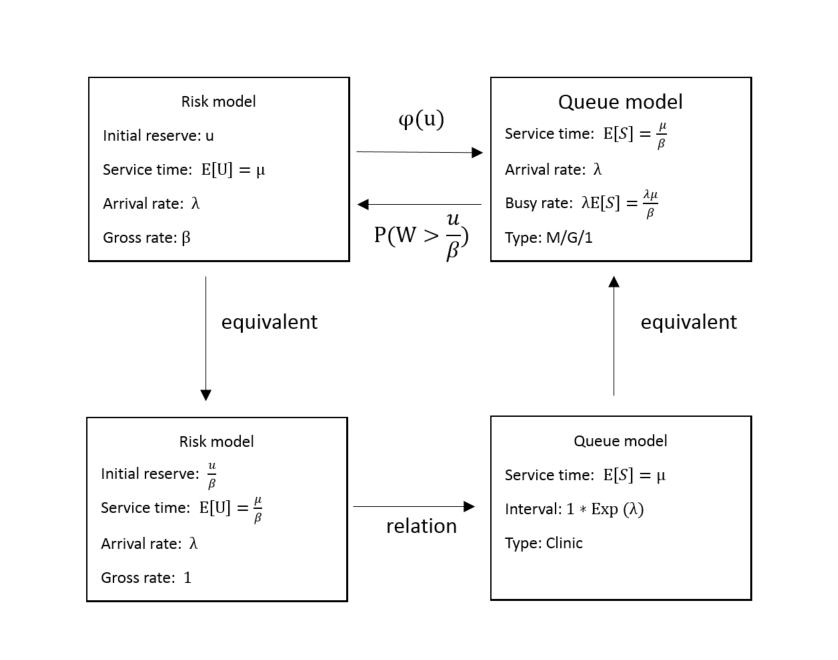
\includegraphics[scale=1]{relation.png}
\caption{Relation between models}
\end{figure}
From figure 1, it is like a new insurer with initial reserve $\frac{u}{\beta}$, {\it gross premium rate =1} and claim size being $\beta$ times smaller than original model. We can construct a clinic model with this new risk model and link the clinic model to the M/G/1 queue.\footnote{NPC implies $\beta>\lambda\mu$ so $\rho=\lambda E[s]=\lambda\frac{\mu}{\beta}<1$, the system can reach equilibrium} So we have
\begin{align*}
\varphi(u)&=\varphi '(\frac{u}{\beta})\\
&=P(\text{Patients waiting time} > \frac{u}{\beta})\\
&=1-P(\text{Waing time} \leq \frac{u}{\beta} \text{ in a M/G/1 queue})
\end{align*}
We can use the Pollaczek-Khinchine formula for waiting time distribution to calculate the ruin probability.!
\begin{theorem}With a random variable R, W is actually a compound distribution
$$\hat{L}_W(s)=\frac{1-\rho}{1-\rho\hat{L}_R(s)}$$
\begin{equation*}
W= \left\{
\begin{array}{lcl}
\sum^{N}_{i=1} R_i  &if N\geq 1,\\
 0 &if N=0,\\
\end{array} 
\right.
\end{equation*}
Where R has density $\frac{\bar{F}_S(t)}{E[s]}$ and $P(N=i)=(1-\rho)(\rho)^i$
\end{theorem}
\begin{proof}
We can rewrite the Laplace transform,
\begin{align*}
\hat{L}_W(s)=\frac{s(1-\rho)}{s-\lambda+\lambda\hat{L}_S(s)}&=\frac{s(1-\rho)E[s]}{sE[s]-\lambda E[s]+\lambda\hat{L}_S(s)E[s]}\\
&=\frac{s(1-\rho)E[s]}{sE[s]-\rho+\rho\hat{L}_S(s)}\\
&=\frac{(1-\rho)}{1-\rho(\frac{1-\hat{L}_S(s)}{sE[s]})}\\
\end{align*} 
From footnote VI, the Laplace transform of R equals $$\hat{L}_R(s)=\frac{1-\hat{L}_S(s)}{sE[s]}$$
Also,
\begin{align*}
\hat{L}_W(s)&=\frac{1-\rho}{1-\rho\hat{L}_R(s)}\\
&=\sum_{i=0}^{\infty}(1-\rho)(\rho)^i(\hat{L}_R(s))^i\\
&=\hat{G}_N(\hat{L}_R(s))
\end{align*} 
By theorem 3, we know W is compound geometric distributed.
\begin{remark}
R is actually the the integral tail distribution we had already used in section 2.2. And, 
\begin{align*}
F_R(z)=F_S^I(z)&=\frac{1}{E[s]}\int_0^z(1-F_S(x))dx\\
&=\frac{1}{\frac{\mu}{\beta}}\int_0^z(1-F_U(\beta x))dx\\
&=\frac{1}{\mu}\int_0^{\beta z}(1-F_U(t))dt=F_U^I(\beta z)\\
\end{align*}
\end{remark}
Applying theorem 2, we have
\begin{align*}
\varphi(u)&=1-F_W(\frac{u}{\beta})\\
&=1-\sum_{i=0}^\infty(1-\rho)(\rho)^i(F_S^I)^{*i}(\frac{u}{\beta})\\
&=1-(1-\rho)-\sum_{i=1}^\infty(1-\rho)(\rho)^i(F_S^I)^{*i}(\frac{u}{\beta})\\
&=\sum_{i=1}^\infty(1-\rho)(\rho)^i-\sum_{i=1}^\infty(1-\rho)(\rho)^i(F_S^I)^{*i}(\frac{u}{\beta})\\
&=\sum_{i=1}^\infty(1-\rho)(\rho)^i(1-(F_S^I)^{*i}(\frac{u}{\beta}))\\
&=(1-\frac{\lambda\mu}{\beta})\sum^{\infty}_{n=1}(\frac{\lambda\mu}{\beta})^n(1-(F_U^I)^{*n}(u))\\
\end{align*}
\end{proof}
This is just as the answer using Integral equation! And this is why it is also called the Pollaczek-Khinchine formula. Survival probability of ruin is just like waiting time distribution in M/G/1 queue. It sounds that they have nothing in common initially, but they are actually the same. How amazing math could be! 
\end{document}